\chapter{Introduction}
\label{chap:intro}

\textbf{Introduction from paper}

Thin-walled shells are, in general, highly efficient structures. In order to produce reliable designs and to avoid unexpected catastrophic failures, one needs to understand buckling. Buckling occurs in a thin structure under loading, when the structure undergoes an overall change in configuration instead of acting in the primary fashion intended by their designers, leading to the failure of the structures. Physically speaking, buckling in a thin shell occurs, when the shell can absorb a great deal of membrane strain energy without deforming too much but it must deform much more in order to absorb an equivalent amount of bending strain energy. When this stored energy is converted into bending energy, buckling occurs, creating a visible change in the geometry of the shell (typically in the form of several dimples) to accommodate all the energy, e.g., Figure 1. Mathematically speaking, buckling can be interpreted as the instability of the equilibrium state that for a certain load will have two possible trajectories to follow, i.e., when in the stress-strain (or stress-deformation) diagram a bifurcation occurs. This phenomenon is mathematically described as the loss of positivity of the second variation of the total energy of the system. In engineering it is essential to have a good estimate on the critical stress that will trigger buckling. In the present work we revisit the problem of buckling of cylindrical shells under axial compression. In that problem, one starts applying homogeneous load of magnitude $\lambda$ to the top of a cylindrical shell that is resting on a substrate, where $\lambda$ is increased continuously from zero. It is observed that at very small load magnitudes $\lambda,$ the cylindrical shell will undergo a homogeneous deformation with no visible geometric changes. Then at some critical value $\lambda=\lambda(h),$ the shell will buckle, producing a variety of deformation patterns, typically in the form of several (or single) dimples 
[cite{bib:Yoshimura},cite{bib:Bud.Hut.},cite{bib:Bushnell},cite{bib:Lan.Cal.Pal.},cite{bib:Dog.Kli.Zim.Ode.Ara.},cite{bib:Hor.Lor.Pel.},cite{bib:Zhu.Man.Cal.}] 
shown in Figure 1\footnote{The second and the third cylinders are apparently deeper into the post-buckling regime.} The dimple (dimples) typically appear with a "click" and drop in the load magnitude (which corresponds to the bifurcation point), and disappear when unloading the shell. Some less common buckling patterns, such as formation of waves in the longitudinal direction or periodic-like wrinkling are also possible, see [cite{bib:Xu.Mic.}] and Figure 14  of [cite{bib:Xu.Mic.}] for more details.
\begin{figure}
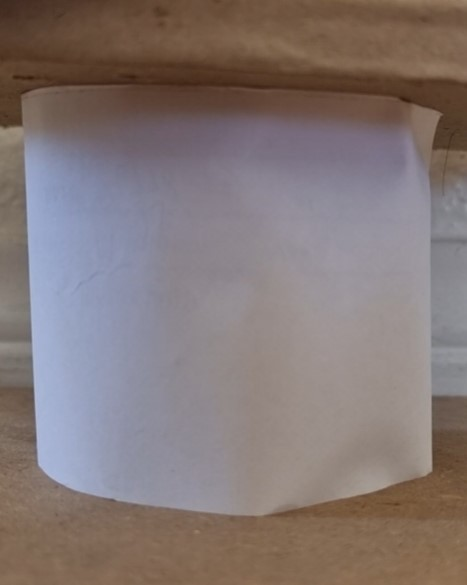
\includegraphics[scale=0.42]{figures/Buckling_1.jpg}\quad

\includegraphics[scale=0.436]{figures/Buckling_2.jpg}\quad
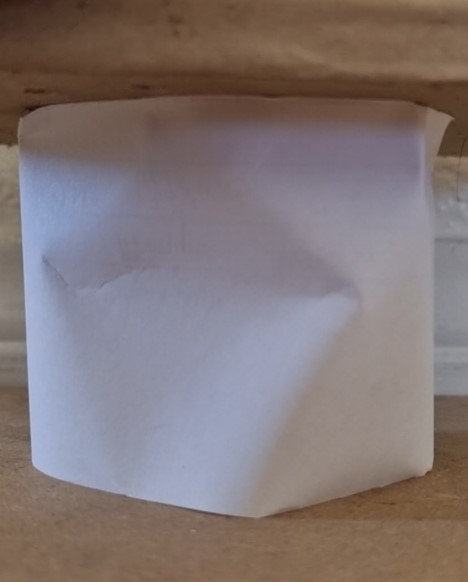
\includegraphics[scale=0.42]{figures/Buckling_3.jpg}\quad
\caption{Buckled paper cylindrical shells under vertical load.}
\end{figure}


Despite being a very old problem with a lot of data available in the literature, (studies and experiments have been made since the mid-18th century), it still contains several unsolved puzzles even for the simplest geometry of perfectly circular cylindrical shells. For the case of circular cylindrical shells, it has been observed that the buckling load measured by experiments has a large discrepancy with the theoretical predictions made by the classical asymptotic formula 
[cite{bib:Lorenz},cite{bib:Timoshenko},cite{bib:Tim.Woi.},cite{bib:Koiter}]
\begin{equation}
\label{1.1}
\lambda(h)=\frac{E h}{\sqrt{3\left(1-\nu^{2}\right)}},
\end{equation}
which predicts a linear relation between the thickness of the cylinder and the critical buckling load $\Gl(h).$ Here $E$ and $\nu$ are the Young modulus and the Poisson ratio of the material, respectively, and $h=t/R$ is the shell dimensionless thickness, i.e., the ratio of the cylinder wall thickness $t$ to the cylinder radius $R$.  Note that in fact formula (\ref{1.1}) was first derived by Lorenz [cite{bib:Lorenz}] in 1911 and independently by Timoshenko [cite{bib:Timoshenko}] in 1914, but  sometimes in the literature it also carries the name of Koiter, as Koiter derived the so-called Koiter circle associated to (\ref{1.1}) in his Ph.D. thesis [cite{bib:Koiter}] in 1945, see also [cite{bib:Gra.Har.3}] for Koiter's circle. On the experimental side, a great deal of experiments since the 1930's show that the experimental critical stress is actually much lower than the theoretical formula (\ref{1.1}), scaling like $h^{3/2}$ with $h$, e.g., [cite{bib:Lan.Cal.Pal.},cite{bib:Zhu.Man.Cal.}]. It has been believed in the engineering and applied mathematics communities, that such a paradoxical behavior is in general due to the fact that the buckling load may be highly sensitive to shape or load imperfections [cite{bib:Almroth},cite{bib:Tennyson},cite{bib:Wei.Mor.Sei.},cite{bib:Gor.Eva.},cite{bib:Yamaki},cite{bib:Hun.Lor.Pel.},cite{bib:Hun.Net.1},cite{bib:Hun.Net.2},cite{bib:Lor.Cha.Hun.}]. Note that \textit{general geometric symmetry breaking or (even a very small) preexisting deformation have been believed to be important factors in the asymptotics of the critical buckling load.} These questions have been addressed in the works [cite{bib:Calladine},cite{bib:Hor.Lor.Pel.},cite{bib:Lan.Cal.Pal.},cite{bib:Zhu.Man.Cal.}] in an attempt to resolve the paradox using mainly numerical approach and/or reduced shell theory equations. One possible gap in these approaches may be whether the utilized reduced shell theory equations are indeed applicable to the problem under consideration and capture the sought parameters within the acceptable error. This concern is based in particular on the works [cite{bib:Fri.Jam.Mor.Mue.},cite{bib:Hor.Lew.Pak.},cite{bib:Lew.Mor.Pak.}], that reveal whether a specific reduced shell theory holds in a specific applied load and elastic energy regime. In the meantime the answer to those specific and important question is unknown. Another weakness was the presence of some heuristic arguments. On the other hand, on the rigorous side, Grabovsky and the first author rigorously proved in [cite{bib:Gra.Har.3}] that indeed Koiter's asymptotic formula (\ref{1.1}) must hold in the case of perfect cylindrical shells and perfect axial homogeneous loading. This was achieved by the improvement and application of the "Thin structure buckling theory" by Grabovsky and Truskinovsky [cite{bib:Gra.Tru.}]. Another crucial component of the analysis in [cite{bib:Gra.Har.3}] was the derivation of the optimal asymptotic constants (not only the asymptotics, but also the leading term in it) in Korn and generalized Korn inequalities for circular cylindrical shells. Then Grabovsky and the first author went on to prove in [cite{bib:Gra.Har.2}] that in fact if even a very small twist (in the angular direction) is present in the shell loading, then the asymptotics of the buckling load has to drop to $h^{5/4},$ see Table 1 below.

\begin{table}[h]
\centering
\resizebox{\textwidth}{!}{%
\begin{tabular}{|l|c|c|}
\hline
\multicolumn{1}{|c|}{Cross-section (C.-S.) and load} & Circular C.-S., vertical load & Circular C.-S., twist in the load \rule{0pt}{4ex}\\ 
 & $\bm\alpha(\theta)=(\cos(\theta),\sin(\theta))$,  $\Bt=-\lambda\bm e_z$ & $\bm\alpha(\theta)=(\cos(\theta),\sin(\theta))$,  $\Bt=-\lambda(\bm e_z+\epsilon \bm e_\theta)$ \rule{0pt}{2ex}\rule[-2ex]{0pt}{0pt}\\
 \hline
Buckling load asymptotics & $\lambda(h)=\frac{E h}{\sqrt{3\left(1-\nu^{2}\right)}}$ & $\lambda(h)=Ch^{5/4}$ \rule{0pt}{4ex}\rule[-3ex]{0pt}{0pt}\\
\hline
\end{tabular}
}\\
\caption{The dependence of the critical buckling load of circular cylindrical shells on the type of loading. Vertical load versus vertical load with a small twist.}
\end{table}
This analysis to some extent gave an explanation to the fact of sensitivity of the buckling load to load imperfections. Also, a somewhat less rigorous argument in [cite{bib:Gra.Har.2}] demonstrated why one should expect the buckling load to drop to $h^{3/2}$ in the presence of some small dimples in the shell. 

Our task in the present work is the analysis of the "sensitivity to imperfections" problem for some other kind of shape imperfections, that are diversions from the perfect cylindrical shell. Namely, we will consider cylindrical shells, generated by cylindrical surfaces, that are non-circular but have convex cross sections: Two main families will be analyzed. 
\begin{itemize}
\item[(i)] The first family contains cylindrical surfaces with convex cross sections that have uniformly positive curvature (when regarded from the exterior of the curve). An illustrative example of such a curve is given in the left half of Figure 2. 
\item[(ii)] The second family contains cylindrical suraces with convex cross sections that have uniformly positive curvature (when regarded from the exterior of the curve) except from finitely many points on the curve, where the curvature vanishes. An illustrative example of such a curve is given in the right half of Figure 2. 
\end{itemize}


\begin{center}
    \begin{figure}
    \centering
    \begin{subfigure}{.48\linewidth}
    \usetikzlibrary {3d}
    \begin{tikzpicture}
     
    %Base
    \draw[fill=gray, semitransparent] (-3,0,-1) -- (3,0,-1) -- (3,0,4) -- (-3,0,4) -- cycle;
    %\draw [ draw=blue] (3,0,0) circle (1pt);
    \def\cost{0.98}
    \def\sint{-0.198 }
    \def\t{0,2}
    %top
     \draw[line width=2pt,domain=-pi:pi]   plot ({2*1.23*cos(\x r)},5,{1.8*sin(\x r)+1.5});
    
    %bottom
      \draw[line width=2pt,domain=-0.25:pi-0.2]   plot ({2*1.23*cos(\x r)},0,{1.8*sin(\x r)+1.5});
    %back bottom
     \draw[line width=2pt,dashed,domain=-0.25-pi:-0.2]   plot ({2*1.23*cos(\x r)},0,{1.8*sin(\x r)+1.5});
    
    %side
    \draw [line width=2pt](-\cost*2*5^0.5+2,5,-\sint*5^0.5+1.5) -- (-\cost*2*5^0.5+2,0,-\sint*5^0.5+1.5);
    \draw [line width=2pt](\cost*2*5^0.5-2,5,\sint*5^0.5+1.5) -- (\cost*2*5^0.5-2,0,\sint*5^0.5+1.5);
    
    
    %Arrows
    \def\top{6}
    \def\tip{5.1}
    %\def\cost{1}
    %\def\sint{0 }
    \draw[-{Latex[length=15pt]}, line width=4pt]({2*1.23*\cost},\top,{-1.8*\sint+1.5})-- ({2*1.23*\cost},\tip,{-1.8*\sint+1.5});
    \draw[-{Latex[length=15pt]}, line width=4pt]({-2*1.23*\cost},\top,{1.8*\sint+1.5})-- ({-2*1.23*\cost},\tip,{1.8*\sint+1.5});
    
    \def\cost{0.866}
    \def\sint{0.5}
    \draw[-{Latex[length=15pt]}, line width=4pt]({2*1.23*\cost},\top,{1.8*\sint+1.5})-- ({2*1.23*\cost},\tip,{1.8*\sint+1.5});
    \draw[-{Latex[length=15pt]}, line width=4pt]({-2*1.23*\cost},\top,{1.8*\sint+1.5})-- ({-2*1.23*\cost},\tip,{1.8*\sint+1.5});
    \draw[-{Latex[length=15pt]}, line width=4pt]({2*1.23*\cost},\top,{-1.8*\sint+1.5})-- ({2*1.23*\cost},\tip,{-1.8*\sint+1.5});
    \draw[-{Latex[length=15pt]}, line width=4pt]({-2*1.23*\cost},\top,{-1.8*\sint+1.5})-- ({-2*1.23*\cost},\tip,{-1.8*\sint+1.5});
    
    \def\cost{0.5}
    \def\sint{0.866}
    \draw[-{Latex[length=15pt]}, line width=4pt]({2*1.23*\cost},\top,{1.8*\sint+1.5})-- ({2*1.23*\cost},\tip,{1.8*\sint+1.5});
    \draw[-{Latex[length=15pt]}, line width=4pt]({-2*1.23*\cost},\top,{1.8*\sint+1.5})-- ({-2*1.23*\cost},\tip,{1.8*\sint+1.5});
    \draw[-{Latex[length=15pt]}, line width=4pt]({2*1.23*\cost},\top,{-1.8*\sint+1.5})-- ({2*1.23*\cost},\tip,{-1.8*\sint+1.5});
    \draw[-{Latex[length=15pt]}, line width=4pt]({-2*1.23*\cost},\top,{-1.8*\sint+1.5})-- ({-2*1.23*\cost},\tip,{-1.8*\sint+1.5});
    \def\cost{0}
    \def\sint{1}
    \draw[-{Latex[length=15pt]}, line width=4pt]({2*1.23*\cost},\top,{1.8*\sint+1.5})-- ({2*1.23*\cost},\tip,{1.8*\sint+1.5});
    \draw[-{Latex[length=15pt]}, line width=4pt]({-2*1.23*\cost},\top,{-1.8*\sint+1.5})-- ({-2*1.23*\cost},\tip,{-1.8*\sint+1.5});
    
    
     \draw[line width=0.2pt,domain=-pi:pi]   plot ({2*1.23*cos(\x r)},\top,{1.8*sin(\x r)+1.5});
     \draw[line width=0.2pt,domain=-pi:pi]   plot ({2*1.23*cos(\x r)},\tip,{1.8*sin(\x r)+1.5});
    
     
    \end{tikzpicture}
    
    \caption{Case (i) in Theorem 3.1: uniformly positive positive curvature, $k_\theta>k>0$}
    \end{subfigure}%
    \hspace{0.5cm}
    \begin{subfigure}{.45\textwidth}
    %\includegraphics[scale=1]{0Curvature.jpg}
    %\centering
    \usetikzlibrary {3d}
    \begin{tikzpicture}
     
    %Base
    \draw[fill=gray, semitransparent] (-3,0,-1) -- (3,0,-1) -- (3,0,4) -- (-3,0,4) -- cycle;
    %\draw [ draw=blue] (3,0,0) circle (1pt);
    \def\cost{0.98}
    \def\sint{-0.198 }
    \def\t{0,2}
    %top
     \draw[line width=2pt,domain=-0.4636476:0.4636476]   plot ({2*(((-1-1)^2+(1.5-0.5)^2)^0.5*cos(\x r)-1)},5,{((-1-1)^2+(1.5-0.5)^2)^0.5*sin(\x r)+1.5});
     \draw[line width=2pt,domain=pi-0.4636476:pi+0.4636476]   plot ({2*(((-1-1)^2+(1.5-0.5)^2)^0.5*cos(\x r)+1)},5,{((-1-1)^2+(1.5-0.5)^2)^0.5*sin(\x r)+1.5});
     \draw[line width=2pt,black, domain=-1:1]   plot (2*\x,5,\x^2*\x^2/2);
     \draw[line width=2pt,black, domain=-1:1]   plot (2*\x,5,-\x^2*\x^2/2+3);
    
    %bottom
     \draw[line width=2pt,domain=-0.2:0.4636476]   plot ({2*(((-1-1)^2+(1.5-0.5)^2)^0.5*cos(\x r)-1)},0,{((-1-1)^2+(1.5-0.5)^2)^0.5*sin(\x r)+1.5});
     \draw[line width=2pt,domain=pi-0.4636476:pi-0.2]   plot ({2*(((-1-1)^2+(1.5-0.5)^2)^0.5*cos(\x r)+1)},0,{((-1-1)^2+(1.5-0.5)^2)^0.5*sin(\x r)+1.5});
     \draw[line width=2pt,black, domain=-1:1]   plot (2*\x,0,-\x^2*\x^2/2+3);
    %back bottom
    \draw[line width=2pt,dashed, domain=-1:1]   plot (2*\x,0,\x^2*\x^2/2);
    \draw[line width=2pt,dashed, domain=-0.4636476:-0.2]   plot ({2*(((-1-1)^2+(1.5-0.5)^2)^0.5*cos(\x r)-1)},0,{((-1-1)^2+(1.5-0.5)^2)^0.5*sin(\x r)+1.5});
    \draw[line width=2pt,dashed, domain=pi-0.2:pi+0.4636476]   plot ({2*(((-1-1)^2+(1.5-0.5)^2)^0.5*cos(\x r)+1)},0,{((-1-1)^2+(1.5-0.5)^2)^0.5*sin(\x r)+1.5});
    %Side
    \draw [line width=2pt](-\cost*2*5^0.5+2,5,-\sint*5^0.5+1.5) -- (-\cost*2*5^0.5+2,0,-\sint*5^0.5+1.5);
    \draw [line width=2pt](\cost*2*5^0.5-2,5,\sint*5^0.5+1.5) -- (\cost*2*5^0.5-2,0,\sint*5^0.5+1.5);
    
    \draw [line width=1pt ] (0,0,3)-- node[above=1mm, rotate = 90] {\large{$\boldsymbol{k}\mathbf{(\theta_0)=0}$} } (0,5,3);
    %\draw (1,-0.5,0) node[anchor=north west] {{{\footnotesize{\color{black}$k(\theta_0)=0$}}}};
    
    
    %Arrows
    \def\top{6}
    \def\tip{5.1}
    
    \draw[-{Latex[length=15pt]}, line width=4pt] (-\cost*2*5^0.5+2,\top,\sint*5^0.5+1.5) -- (-\cost*2*5^0.5+2,\tip,\sint*5^0.5+1.5);
    \draw[-{Latex[length=15pt]}, line width=4pt] (+\cost*2*5^0.5-2,\top,-\sint*5^0.5+1.5) -- (+\cost*2*5^0.5-2,\tip,-\sint*5^0.5+1.5);
    \def\t{-1}
    \draw[-{Latex[length=15pt]}, line width=4pt] (2*\t,\top,\t^2*\t^2/2)-- (2*\t,\tip,\t^2*\t^2/2);
    \draw[-{Latex[length=15pt]}, line width=4pt] (2*\t,\top,-\t^2*\t^2/2+3)-- (2*\t,\tip,-\t^2*\t^2/2+3);
    \def\t{-0.5}
    \draw[-{Latex[length=15pt]}, line width=4pt] (2*\t,\top,\t^2*\t^2/2)-- (2*\t,\tip,\t^2*\t^2/2);
    \draw[-{Latex[length=15pt]}, line width=4pt] (2*\t,\top,-\t^2*\t^2/2+3)-- (2*\t,\tip,-\t^2*\t^2/2+3);
    \def\t{0}
    \draw[-{Latex[length=15pt]}, line width=4pt] (2*\t,\top,\t^2*\t^2/2)-- (2*\t,\tip,\t^2*\t^2/2);
    \draw[-{Latex[length=15pt]}, line width=4pt] (2*\t,\top,-\t^2*\t^2/2+3)-- (2*\t,\tip,-\t^2*\t^2/2+3);
    \def\t{0.5}
    \draw[-{Latex[length=15pt]}, line width=4pt] (2*\t,\top,\t^2*\t^2/2)-- (2*\t,\tip,\t^2*\t^2/2);
    \draw[-{Latex[length=15pt]}, line width=4pt] (2*\t,\top,-\t^2*\t^2/2+3)-- (2*\t,\tip,-\t^2*\t^2/2+3);
    \def\t{1}
    \draw[-{Latex[length=15pt]}, line width=4pt] (2*\t,\top,\t^2*\t^2/2)-- (2*\t,\tip,\t^2*\t^2/2);
    \draw[-{Latex[length=15pt]}, line width=4pt] (2*\t,\top,-\t^2*\t^2/2+3)-- (2*\t,\tip,-\t^2*\t^2/2+3);
    
    %top
     \draw[line width=0.2pt,domain=-0.4636476:0.4636476]   plot ({2*(((-1-1)^2+(1.5-0.5)^2)^0.5*cos(\x r)-1)},\tip,{((-1-1)^2+(1.5-0.5)^2)^0.5*sin(\x r)+1.5});
     \draw[line width=0.2pt,domain=pi-0.4636476:pi+0.4636476]   plot ({2*(((-1-1)^2+(1.5-0.5)^2)^0.5*cos(\x r)+1)},\tip,{((-1-1)^2+(1.5-0.5)^2)^0.5*sin(\x r)+1.5});
     \draw[line width=0.2pt,black, domain=-1:1]   plot (2*\x,\tip,\x^2*\x^2/2);
     \draw[line width=0.2pt,black, domain=-1:1]   plot (2*\x,\tip,-\x^2*\x^2/2+3);
    
     \draw[line width=0.2pt,domain=-0.4636476:0.4636476]   plot ({2*(((-1-1)^2+(1.5-0.5)^2)^0.5*cos(\x r)-1)},\top,{((-1-1)^2+(1.5-0.5)^2)^0.5*sin(\x r)+1.5});
     \draw[line width=0.2pt,domain=pi-0.4636476:pi+0.4636476]   plot ({2*(((-1-1)^2+(1.5-0.5)^2)^0.5*cos(\x r)+1)},\top,{((-1-1)^2+(1.5-0.5)^2)^0.5*sin(\x r)+1.5});
     \draw[line width=0.2pt,black, domain=-1:1]   plot (2*\x,\top,\x^2*\x^2/2);
     \draw[line width=0.2pt,black, domain=-1:1]   plot (2*\x,\top,-\x^2*\x^2/2+3);
     %\draw (-0.5,0) node[anchor=north west] {{{\footnotesize{\color{black}$k(\theta_0)=0$}}}};
    \end{tikzpicture}
    
    \caption{Case (ii) in Theorem 3.1: curvature vanish in 2 isolated points. Around $\theta_0$ the curve behaves like $\bm\alpha(\theta)=(\theta, \theta^4).$}
    \end{subfigure}
    \caption{Possible Cross-sections,  with positive curvatures}
    \end{figure}
    \end{center}




Note that in both cases the cylinder cross-section does not have to have any geometric symmetry property, but rather only has to be convex with some imposed curvature condition. We will prove that in case (i) the critical buckling load $\Gl(h)$ has the asymptotics $Ch$, and in case (ii) we will prove the bounds
 $C_1h^{8/5}\leq \Gl(h)\leq C_2h^{3/2}$ in the vanishing thickness regime $h\to 0.$ The result in part (i) in particular disproves the longstanding believe that  geometric symmetry breaking would lead to the drop in the asymptotics of $\Gl(h),$ i.e., there is an $\epsilon>0,$ such that $\Gl(h)\leq Ch^{1+\epsilon}$. Also, the result in part (ii) provides new evidence on how a geometric shape imperfection, which is a diversion from the perfect cylindrical shell may lead to the drop in the asymptotics of $\Gl(h)$ to at least $h^{3/2}.$ 

As already pointed out, we will be working in the framework of the (improved) "thin structure buckling theory" of Grabovsky and Truskinovsky [cite{bib:Gra.Tru.}] rigorously derived from three-dimensional nonlinear hyper-elasticity. Some of the main components in the analysis will be asymptotically sharp Korn 
inequalities for the displacement gradient components, proven for the shells under consideration. 

The paper is organized as follows: In Section~2 we present a brief introduction to the general theory of slender structure buckling [cite{bib:Gra.Tru.},cite{bib:Gra.Har.2}]. 
In Section~3 we will be formulating the main results of the paper. In order to apply the theory in Section~2, on one hand one needs to determine 
(with some amount of proximity) the so-called "trivial branch", and the asymptotic stress tensor, which will be done in Section~4.1. Also, on the other hand one needs to prove asymptotically sharp Korn and Korn-type inequalities for the displacement gradient components, thus in Sections~4.2-4.3 we will formulate and prove those. Finally, in Section~4.4 we will prove the main results on the buckling load. 
